\documentclass{article}
\usepackage{longtable}
\usepackage{makecell}
\usepackage{float}
\usepackage{graphicx}
\usepackage{bm}
\usepackage{placeins}
\usepackage{booktabs}
\usepackage{gensymb}
\usepackage{amssymb}
\usepackage{indentfirst}
\usepackage{threeparttable} 
\usepackage{multirow}
\usepackage{aligned-overset}
\usepackage[slantfont,boldfont]{xeCJK}
\usepackage{fontspec}
\renewcommand{\arraystretch}{1.5}
\usepackage[paperwidth=23cm,paperheight=37.21cm]{geometry}
\setCJKmainfont{SimSun}
\setmainfont{SimSun}
\setsansfont{SimSun}

\title{杨氏模量测定实验报告}
\author{2411545 邱凯锐}
\date{2025.4.28}

\begin{document}
\maketitle
\section{实验目的}
1.用伸长法测定金属丝的杨氏模量;

2.了解望远镜的结构和使用方法;

3.掌握用光杠杆测量微小长度变化量的方法;

4.学习用对立影响法消除系统误差的思想方法;

5.用环差法处理数据;

\section{实验仪器}
杨氏模量测定仪、千分尺、游标卡尺、米尺及照明光源等。

杨氏模量测定仪主要包括伸长仪、光杠杆、平面反射和望远镜尺组四个部分。

1. \textbf{伸长仪}

如图 8 - 1 所示,它是一双立柱三角支架,由固定螺钉固定着待测金属丝,待测金属丝的下端与小圆柱连接,小圆柱穿过载物平台的中心孔,其下端悬挂砝码托。当金属丝受力伸长时,小圆柱能在圆孔中无摩擦地下移。载物平台上放置光杠杆,光杠杆前端两个足尖(或刀片)被置于载物平台的沟槽内,后端的一个足尖被置于和待测金属丝连在一起的小圆柱上,并随之升降。底脚螺丝用以调节立柱铅直,铅直度可由铅垂线或靠目测判断。

2. \textbf{光杠杆和望远镜尺组}
    
(1)光杠杆。直立的平面反射镜通过两个紧固螺丝安装在底盘的一端,底盘下固定着两个前足尖(或刀刃)被置于伸长仪载物平台的“V”形槽中,另一端为后足尖,后足尖应与两个前足尖构成等腰
三角形,该等腰三角形的高\(b\)称为光杠杆常数。松开臂长调节螺丝(图中未表示出),可以根据需要改变光杠杆常数。松开固定螺丝,可以调节平面反射镜的铅直度。

(2) 望远镜。它由内调焦望远镜和米尺组合而成。通过望远镜及米尺固定旋钮可分别改变它们在三角架立柱上的高度;通过米尺调整螺丝还可以改变标尺与其支架的相对位置;立柱铅直度靠其地脚螺丝调节(目测)。使用时,先取下物镜罩,调节目镜的视度圈,使分划板刻线清晰;移动镜尺组三角架或松开望远镜固定旋钮以调节其高度或角度,使镜筒对准待观测目标(如米尺在反射镜中的像);调节目镜下侧附近的微动手轮,从目镜端以准星仔细瞄准目标;最后调节内调焦手轮,调整视距,直至被观测目标(米尺)在视场中心且成像清晰为止。

\begin{figure}
    \centering
    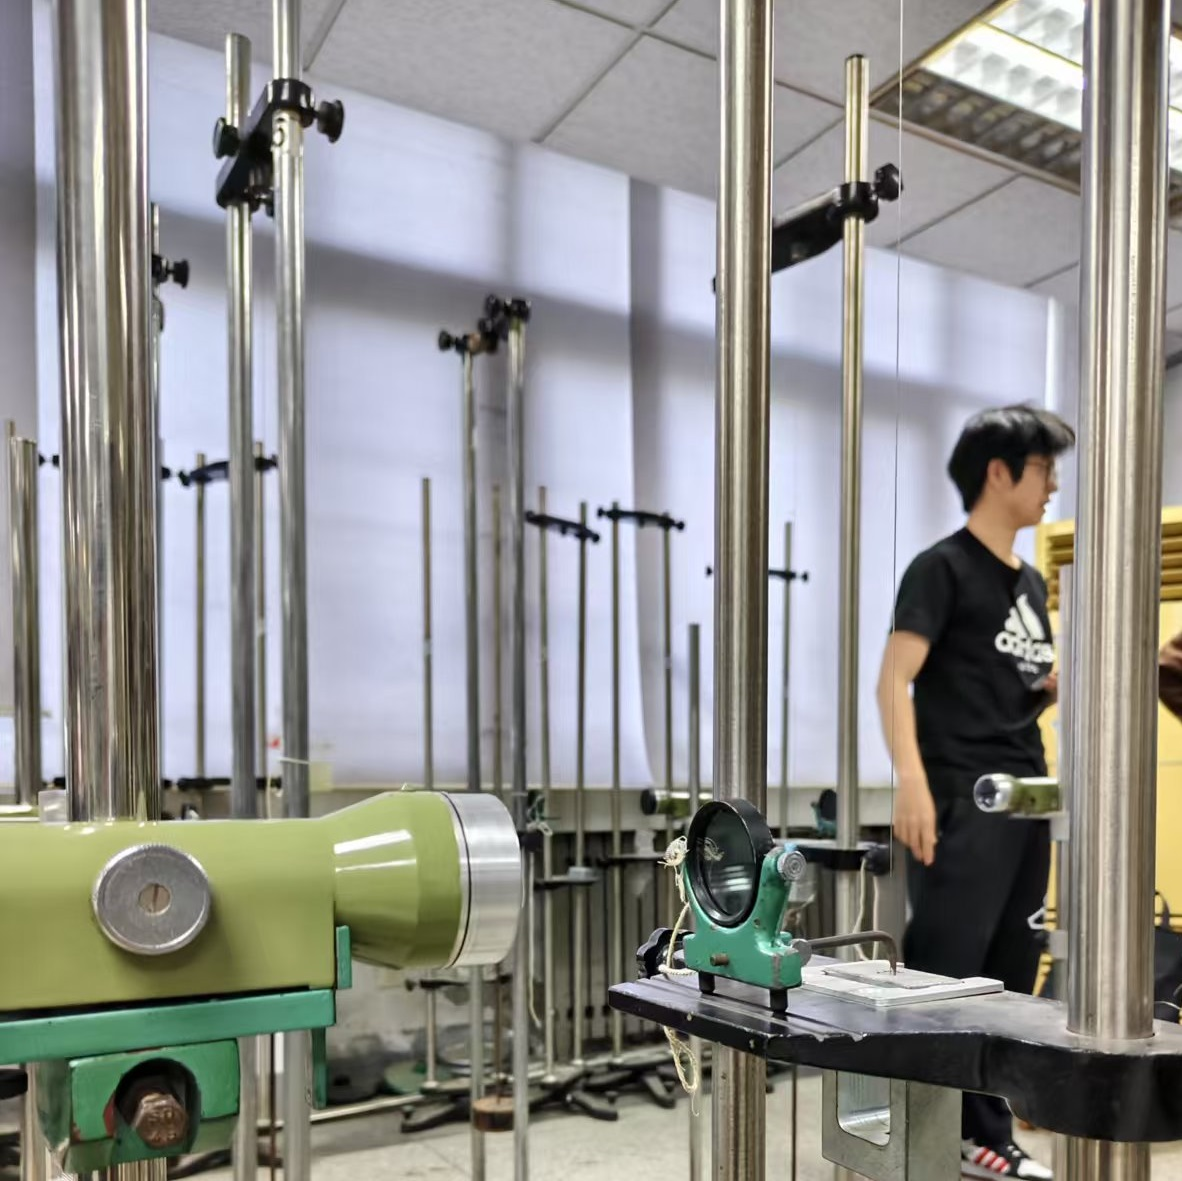
\includegraphics[width=6cm]{1.jpg}
    \caption{实验装置}
\end{figure}

\section{实验原理}
若长 \(l\)、截面积 \(S\) 均匀的金属丝或棒,在其长度方向上受到作用力 \(F\) 而伸长 \(\Delta l\),则据虎克定律:在弹性限度内,胁强 \(F/S\) 与协变 \(\Delta l/l\) 成正比,即:

\begin{equation}
\frac{F}{S}=E\cdot\frac{\Delta l}{l}
\end{equation}

式 \((1)\) 中比例系数 \(E\) 即为该金属材料的杨氏模量。将式 \((1)\) 改写为:

\begin{equation}
E = \frac{Fl}{S\Delta l}
\end{equation}

在式\((2)\)中,\(F\)、\(S\)及\(l\)比较容易测量,由于金属的杨氏模量一般较大,因此,\(\Delta l\)是一个微小的长度变化,很难用普通测量长度的仪器将它测准。因此,实验装置的主要部分就是为了解决这个微小长度变化量的测量。光杠杆和望远镜尺组为其测量提供了方便。

\begin{figure}[ht]
    \centering
    \begin{minipage}{0.45\textwidth} % 调整宽度为总宽度的45%
        \centering
        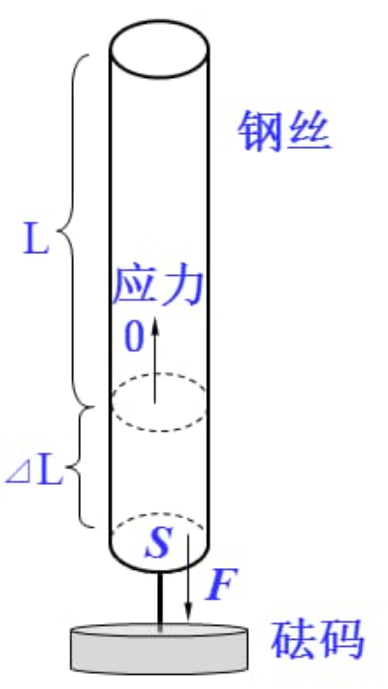
\includegraphics[width=3cm]{3.png} % 替换为你的图片路径
        \caption{杨氏模量定义图}
    \end{minipage}\hfill
    \begin{minipage}{0.45\textwidth}
        \centering
        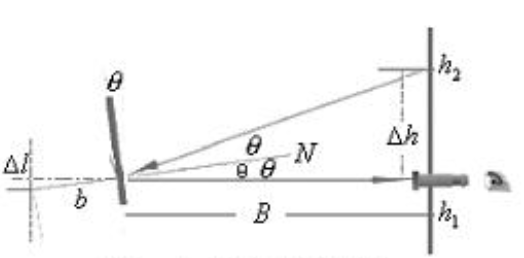
\includegraphics[width=7cm]{2.png} % 替换为你的图片路径
        \caption{光杠杆放大原理}
    \end{minipage}
\end{figure}

光杠杆和望远镜尺组二者配合,即可有效地测定金属丝在外力作用下的伸长量\(\Delta l\)。金属丝受力伸长\(\Delta l\),光杠杆后足尖随之下降\(\Delta l\),因其前足尖(刀刃)仍在平台槽底(高度不变),所以,光杠杆连同其镜面以刀刃为轴旋转一角度\(\theta\)。如Figure 3所示,当\(\theta\)角很小时,有

\begin{equation}
    \sin\theta = \frac{\Delta l}{b} \approx \theta
\end{equation}

据几何光学反射定律,当平面镜偏转\(\theta\)角度时,只有与原入射光线成\(2\theta\)角的光线才能进入望远镜被观测到。假定平面镜面至标尺的距离为\(B\),则有:

\begin{equation}
    \tan 2\theta = \frac{h_2 - h_1}{B} = \frac{\Delta h}{B} \approx 2\theta 
\end{equation}

由式(3)及(4)可得

\begin{equation}
    \Delta l = \frac{b \cdot \Delta h}{2B} 
\end{equation}

式(5)表明,光杠杆和镜尺组的作用在于,将微小的长度变化量\(\Delta l\)转变为标尺刻线的像移\(\Delta h\),而\(\Delta h\)比\(\Delta l\)放大了\(\frac{2B}{b}\)倍,这就是光杠杆的放大原理。式(5)成立的条件是:\(\theta\)角很小,光杠杆三足尖在同一水平面内,且平面镜及标尺竖直等,满足了上述条件,即可通过\(b\)、\(B\)及\(\Delta h\)这些比较容易测准的量而间接求出微小变化量\(\Delta l\)。

将式(5)代入式(2),并利用\(S = \frac{\pi D^2}{4}\)及\(F = mg\),可得:

\begin{equation}
    E = \frac{8Blmg}{\pi D^2 b \Delta h} 
\end{equation}

式(8)即为用伸长法测定金属丝杨氏模量的数学表达式。其中,\(D\)表示金属丝直径(其原分布既有不圆度,也有不均匀度);\(g = 9.8m/s^2\)表示重力加速度;\(m\)表示金属丝下端所加砝码的质量。


\section{实验内容与注意事项}
\subsection{实验内容}
1. 调节伸长仪和光杠杆使之达到备用状态;

2. 移动望远镜尺组,使标尺距平面镜略大于\(1m\);调节望远镜的高度及方向,使其与平面镜等高,且其瞄准方向应对正欲观测目标(反射镜中标尺的像); 

3. 以灯光照明标尺,参照望远镜调节及使用方法,迅速准确地找到标尺的像,使成像清晰,且应使分划板准线所对应的标尺刻度数略低于望远镜轴线所在刻度读数。(即使平面镜略呈前倾,相应地后足尖略高出水平面,但反射镜面仍应与光杠杆三足尖所成的平面垂直。) 

4. 观测像移:依次按等时间隔(2分钟左右) 递加砝码\(2kg\),记下相应读数\(h_{i}\),直至\(10kg\);然后仍按等时间隔逐次递减砝码\(2kg\),记下相应读数\(h_{i}^{'}\),取两组读数的平均值\(\overline{h}_{i}=(h_{i}+h_{i}^{'})/2\)作为相应的测量值。这样做的目的是:以对立影响法(或称对称测量方法)消除或减弱金属丝弹性滞后效应及小圆柱与平台间可能的机械摩擦带来的影响。 

5. 以米尺测\(l\)及\(B\)各一次,以千分尺在金属丝不同部位的互垂方向上测直径\(D\)六次; 

6. 测光杠杆常数\(b\)。方法是:将光杠杆放在平纸上,轻印三足尖之痕迹,然后以游标卡尺测量印痕间距离一次。

\subsection{注意事项}
1.保持光学镜面清洁,不得用手触摸,镜面有灰尘时,应以软毛刷轻拭,且用毕应盖好物镜罩;

2.调节望远镜时,动作要轻,且尽量不靠微动手轮瞄准目标,伸长仪及望远镜尺组应避免撞击和剧烈振动;

3.应保护光杠杆刀刃、足尖及平面镜,严禁磕碰和跌落;其固定螺丝不得旋得过紧,以防平面镜变形;

4.测像移过程中不得碰动仪器的任何部位,且加减砝码时动作要轻,防止砝码托摆动,以提高测量精度。

\section{实验数据}
\begin{figure}[!ht]
    \centering
    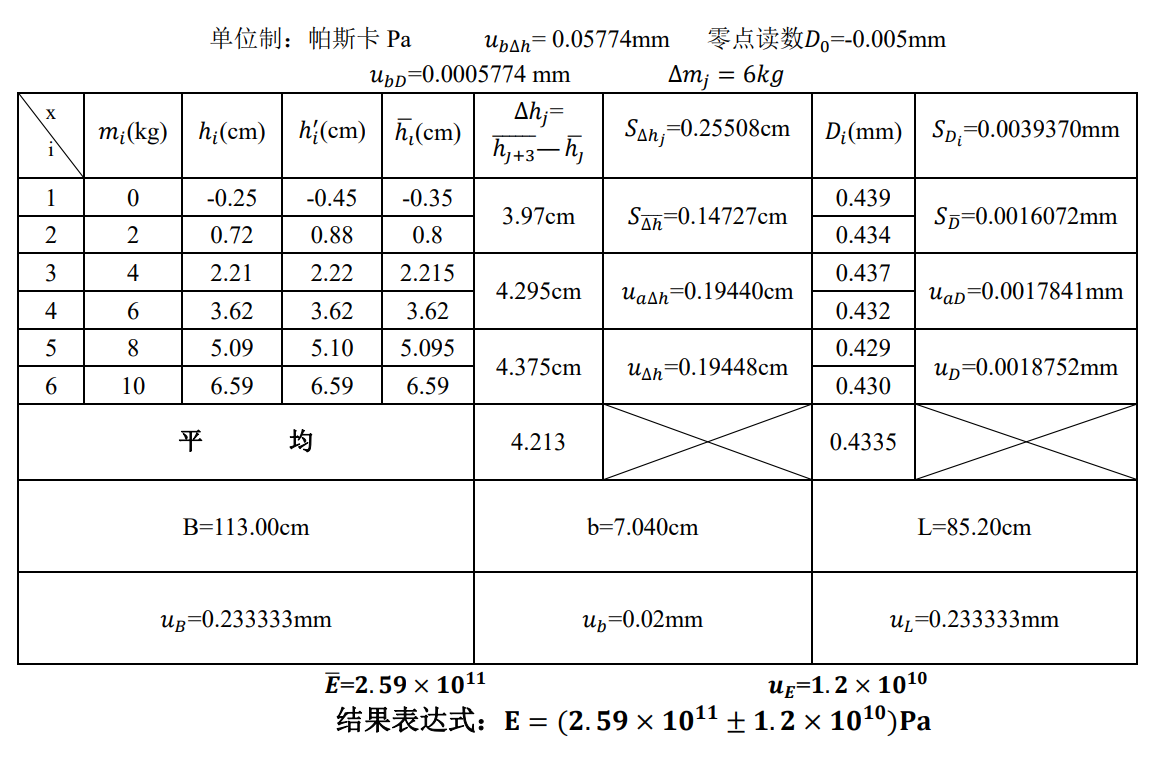
\includegraphics[width=16cm]{data.png}
\end{figure}

\section{实验数据处理}
\subsection{杨氏模量计算}
先运用对立影响法,计算$h_i$和$h_i'$的平均值$\overline{h_i}$,再利用还差法计算$\Delta h_j=\overline{h_{j+3}}-\overline{h_j}$,最后求出平均值$\overline{\Delta h}$。
对于钢丝直径$D_i$求平均值$\overline{D}$。最后将数值代入杨氏模量$E$的表达式中,得到:

$$
\overline{E}=\frac{8BL\Delta m_jg}{\pi\overline{D}^2b\overline{\Delta h}}=\frac{8*1.1300*0.8520*6*9.8}{\pi·(0.4335\times 10^{-3})^2*0.07040*0.04213} Pa=2.588228\times 10^{11} Pa
$$

\subsection{不确定度计算}

对式(6)两边取对数后求全微分得到:

$$
\frac{u_E}{\overline{E}}=\frac{u_B}{B}+\frac{u_L}{L}-\frac{2u_D}{\overline{D}}-\frac{u_b}{b}-\frac{u_{\Delta h}}{\overline{\Delta h}}
$$

从而:

$$
u_E=\overline{E}\cdot\sqrt{(\frac{u_L}{L})^2+(\frac{u_B}{B})^2+(\frac{2u_D}{D})^2+(\frac{u_{\Delta h}}{\Delta h})^2+(\frac{u_b}{b})^2}
$$


对于单次测量量L、B和b。不确定度为:

$$
u_L=\frac{\Delta x}{c}=\frac{0.5mm}{3}\qquad u_B=\frac{\Delta x}{c}=\frac{0.5mm}{3}\qquad u_b=\frac{\Delta x'}{c'}=\frac{0.02mm}{1}
$$

由于读数时存在误差,实际计算时$\Delta x$将增加$0.1mm-0.2mm$。本实验中取$\Delta x=0.7mm$。

对于多次测量量$D$和$h$。以$D$为例,计算标准偏差$S_{\overline{D}}$、A类不确定度$U_{aD}$、B类不确定度$D_{bD}$和不确定度$u_D$:
$$
\overline{S_{D_{i}}}=\sqrt{\frac{\sum_{i = 1}^{6}(D_i-\overline{D})^2}{6-1}}=3.9379\times10^{-3}mm \qquad S_{\overline{D}}=\frac{\overline{S_{D_i}}}{\sqrt{6}}=1.6072\times10^{-3}mm
$$

$$
u_{aD}=t\cdot S_{\overline{D}}=1.7841\times10^{-3}mm,\quad 其中t(0.683,5)=1.11
$$

$$
u_{bD}=\frac{\varepsilon_0}{\sqrt{3}}=5.774\times 10^{-4},\quad 其中\varepsilon_0=0.001mm
$$

$$
u_D=\sqrt{{u_{aD}}^2+{u_{bD}}^2}=1.8752\times10^{-3}mm
$$

对于$h$同理:
$$
\overline{S_{\Delta h_{i}}}=\sqrt{\frac{\sum_{i = 1}^{3}(\Delta h_i-\overline{\Delta h})^2}{6-1}}=2.5508\times10^{-1}cm \qquad S_{\overline{\Delta h}}=\frac{\overline{S_{\Delta h_i}}}{\sqrt{3}}=1.4727\times10^{-1}cm
$$

$$
u_{a\Delta h}=t\cdot S_{\overline{\Delta h}}=1.9440\times10^{-1}cm,\quad 其中t(0.683,2)=1.32
$$

$$
u_{b\Delta h}=\frac{\varepsilon_0}{\sqrt{3}}=5.774\times 10^{-2},\quad 其中\varepsilon_0=0.1mm
$$

$$
u_{\Delta h}=\sqrt{{u_{a\Delta h}}^2+{u_{b \Delta h}}^2}=1.9448\times10^{-1}cm
$$

最后计算杨氏模量的不确定度$u_E$

$$
u_E=\overline{E}\cdot\sqrt{(\frac{u_L}{L})^2+(\frac{u_B}{B})^2+(\frac{2u_D}{D})^2+(\frac{u_{\Delta h}}{\Delta h})^2+(\frac{u_b}{b})^2}=1.2\times{10^{10}} Pa
$$

杨氏模量的结果表达式为:
$$
E=\overline{E}\pm u_E=(2.59\times10^{11}\pm 1.2\times10^{10})Pa
$$

\section{实验结论与误差分析}

本实验的计算结果$E=(2.59\times10^{11}\pm 1.2\times10^{10})Pa$,与给出的标准值$E_{标准}=2\times10^{11}Pa$,较为接近,得到了钢丝的杨氏模量的具体值。

对于误差分析主要由以下几点:

\begin{itemize}
    \item 1.米尺、游标卡尺和螺旋测微计等测量工具精度受限;
    \item 2.环境因素影响,例如:温度变化、空气流动;
    \item 3.操作因素,增加和卸下砝码时使伸长仪发生微小唯一,进而使得光杠杆位置发生变化;
    \item 4.砝码生锈老化,质量发生改变,不严格等于 2kg ;
    \item 5.光杠杆读数误差,读数时与望远镜的视角偏差,系统本身的微小摆动使光杠杆的读数难以非常精确;
    \item 6.仪器校准误差,光杠杆、望远镜和平面反射镜等仪器的安装和调节不准确,使测量结果产生偏差。 
\end{itemize}

\end{document}